\section{Results}\label{sec:results}

\subsection{RMSE}

\subsection{Conservation of Energy}\label{sec:energy_conservation}

By using (INSERT EQUATION REF.) %\eqref{eq:energy-conservation}, 
we can calculate the energy of the system, and in turn can the energy conservation be studied as a function of $dt$. The system used for the energy conservation study was that of a small perturbation in initial velocity from the trivial solution studied previously. 

Firstly was the energy for the system with initial velocity \textbf{less} than the equilibrium velocity studied. Because the system will converge towards the centrepoint, the integration will at some point become singular for this case. Hence was the case that the initial velocity slightly larger than the equilibrium velocity studied. 

In natural units, we define the initial conditions by letting

\begin{align}
	M &= 1 \\
	r &= 6M \\
	v &= \sqrt{\frac{M}{r}} + 0.01 \frac{M}{r} \\
	\dot{\phi} &= rv
\end{align}



The general behavior is that the energy decreases with the time / angle (CHECK BOTH TIME AND ANGLE DEPENDENCE), with a small oscillative form and a trend downwards. The energy decreases the most for 

We fit a linear curve to the curves, and compare the slopes and try to conclude a relationship between them. 

\begin{figure}[!ht]
	\centering
	\begin{subfigure}[b]{0.3\textwidth}
	\centering
	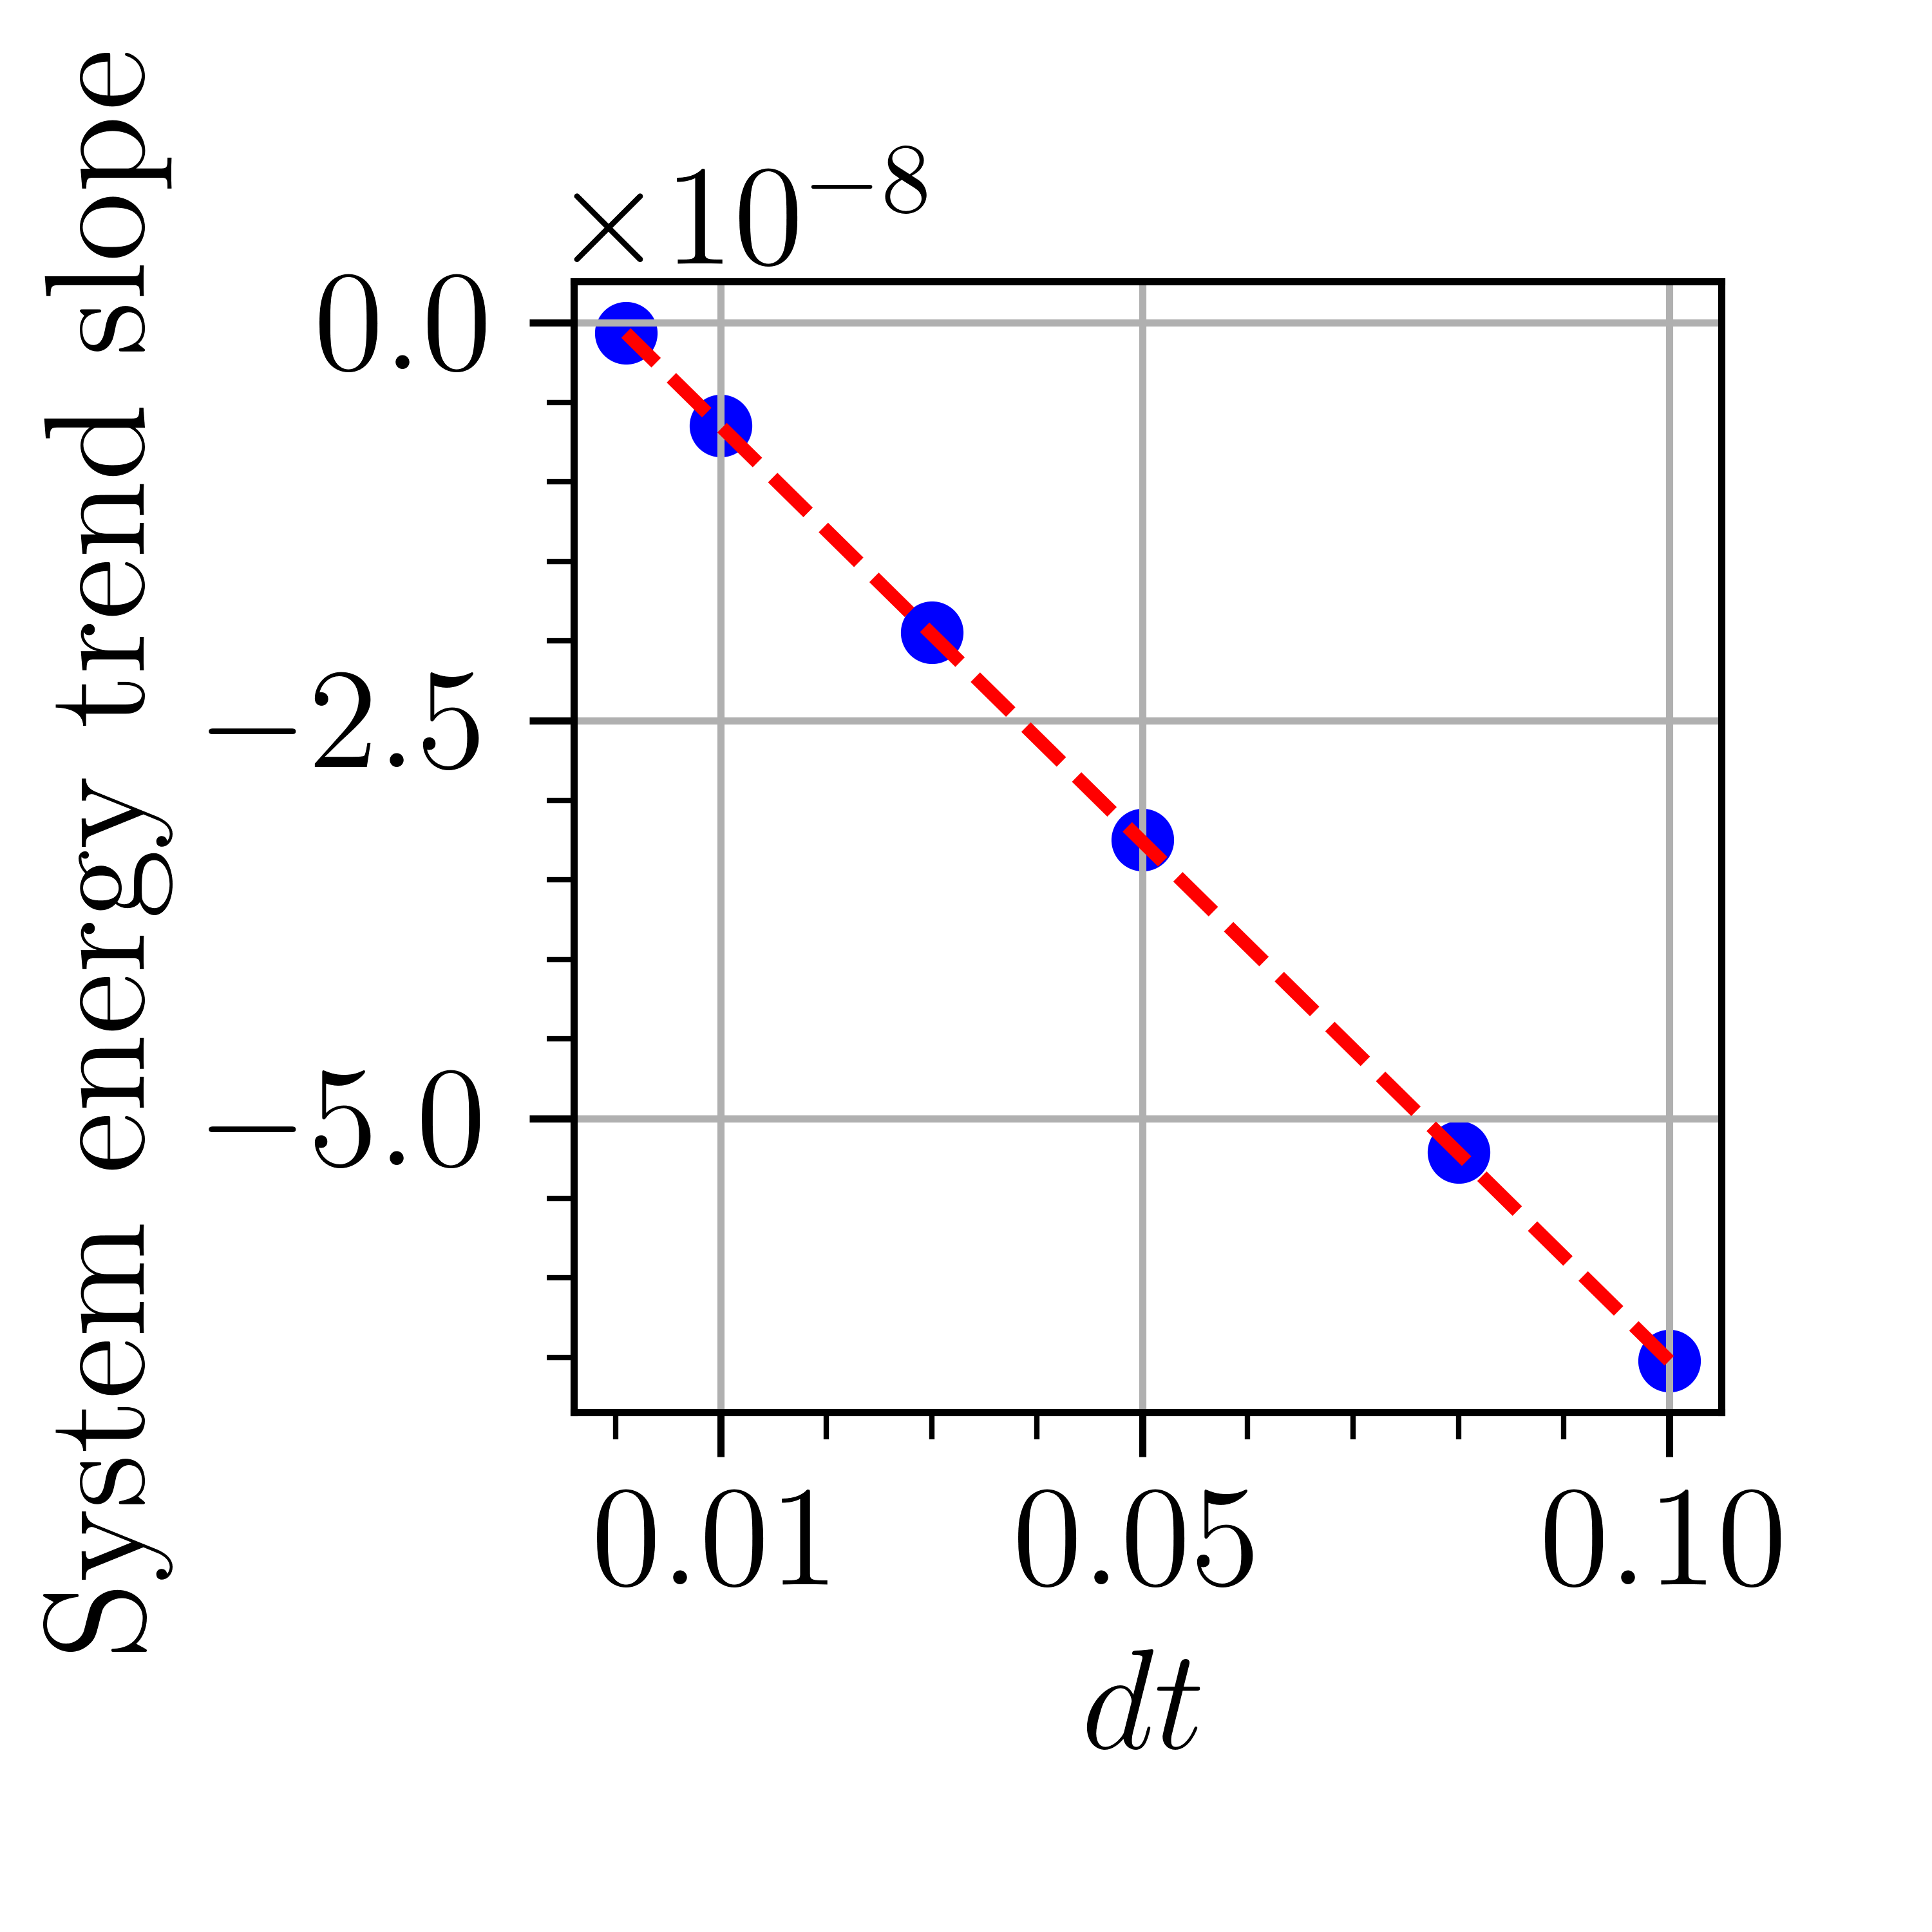
\includegraphics[width=1.0\textwidth]{figures/energy_conservation_euler_method}
	\caption{Euler method}
	\label{fig:energy_cons_euler_method}
	\end{subfigure}
	\hfill
	\begin{subfigure}[b]{0.3\textwidth}
	\centering
	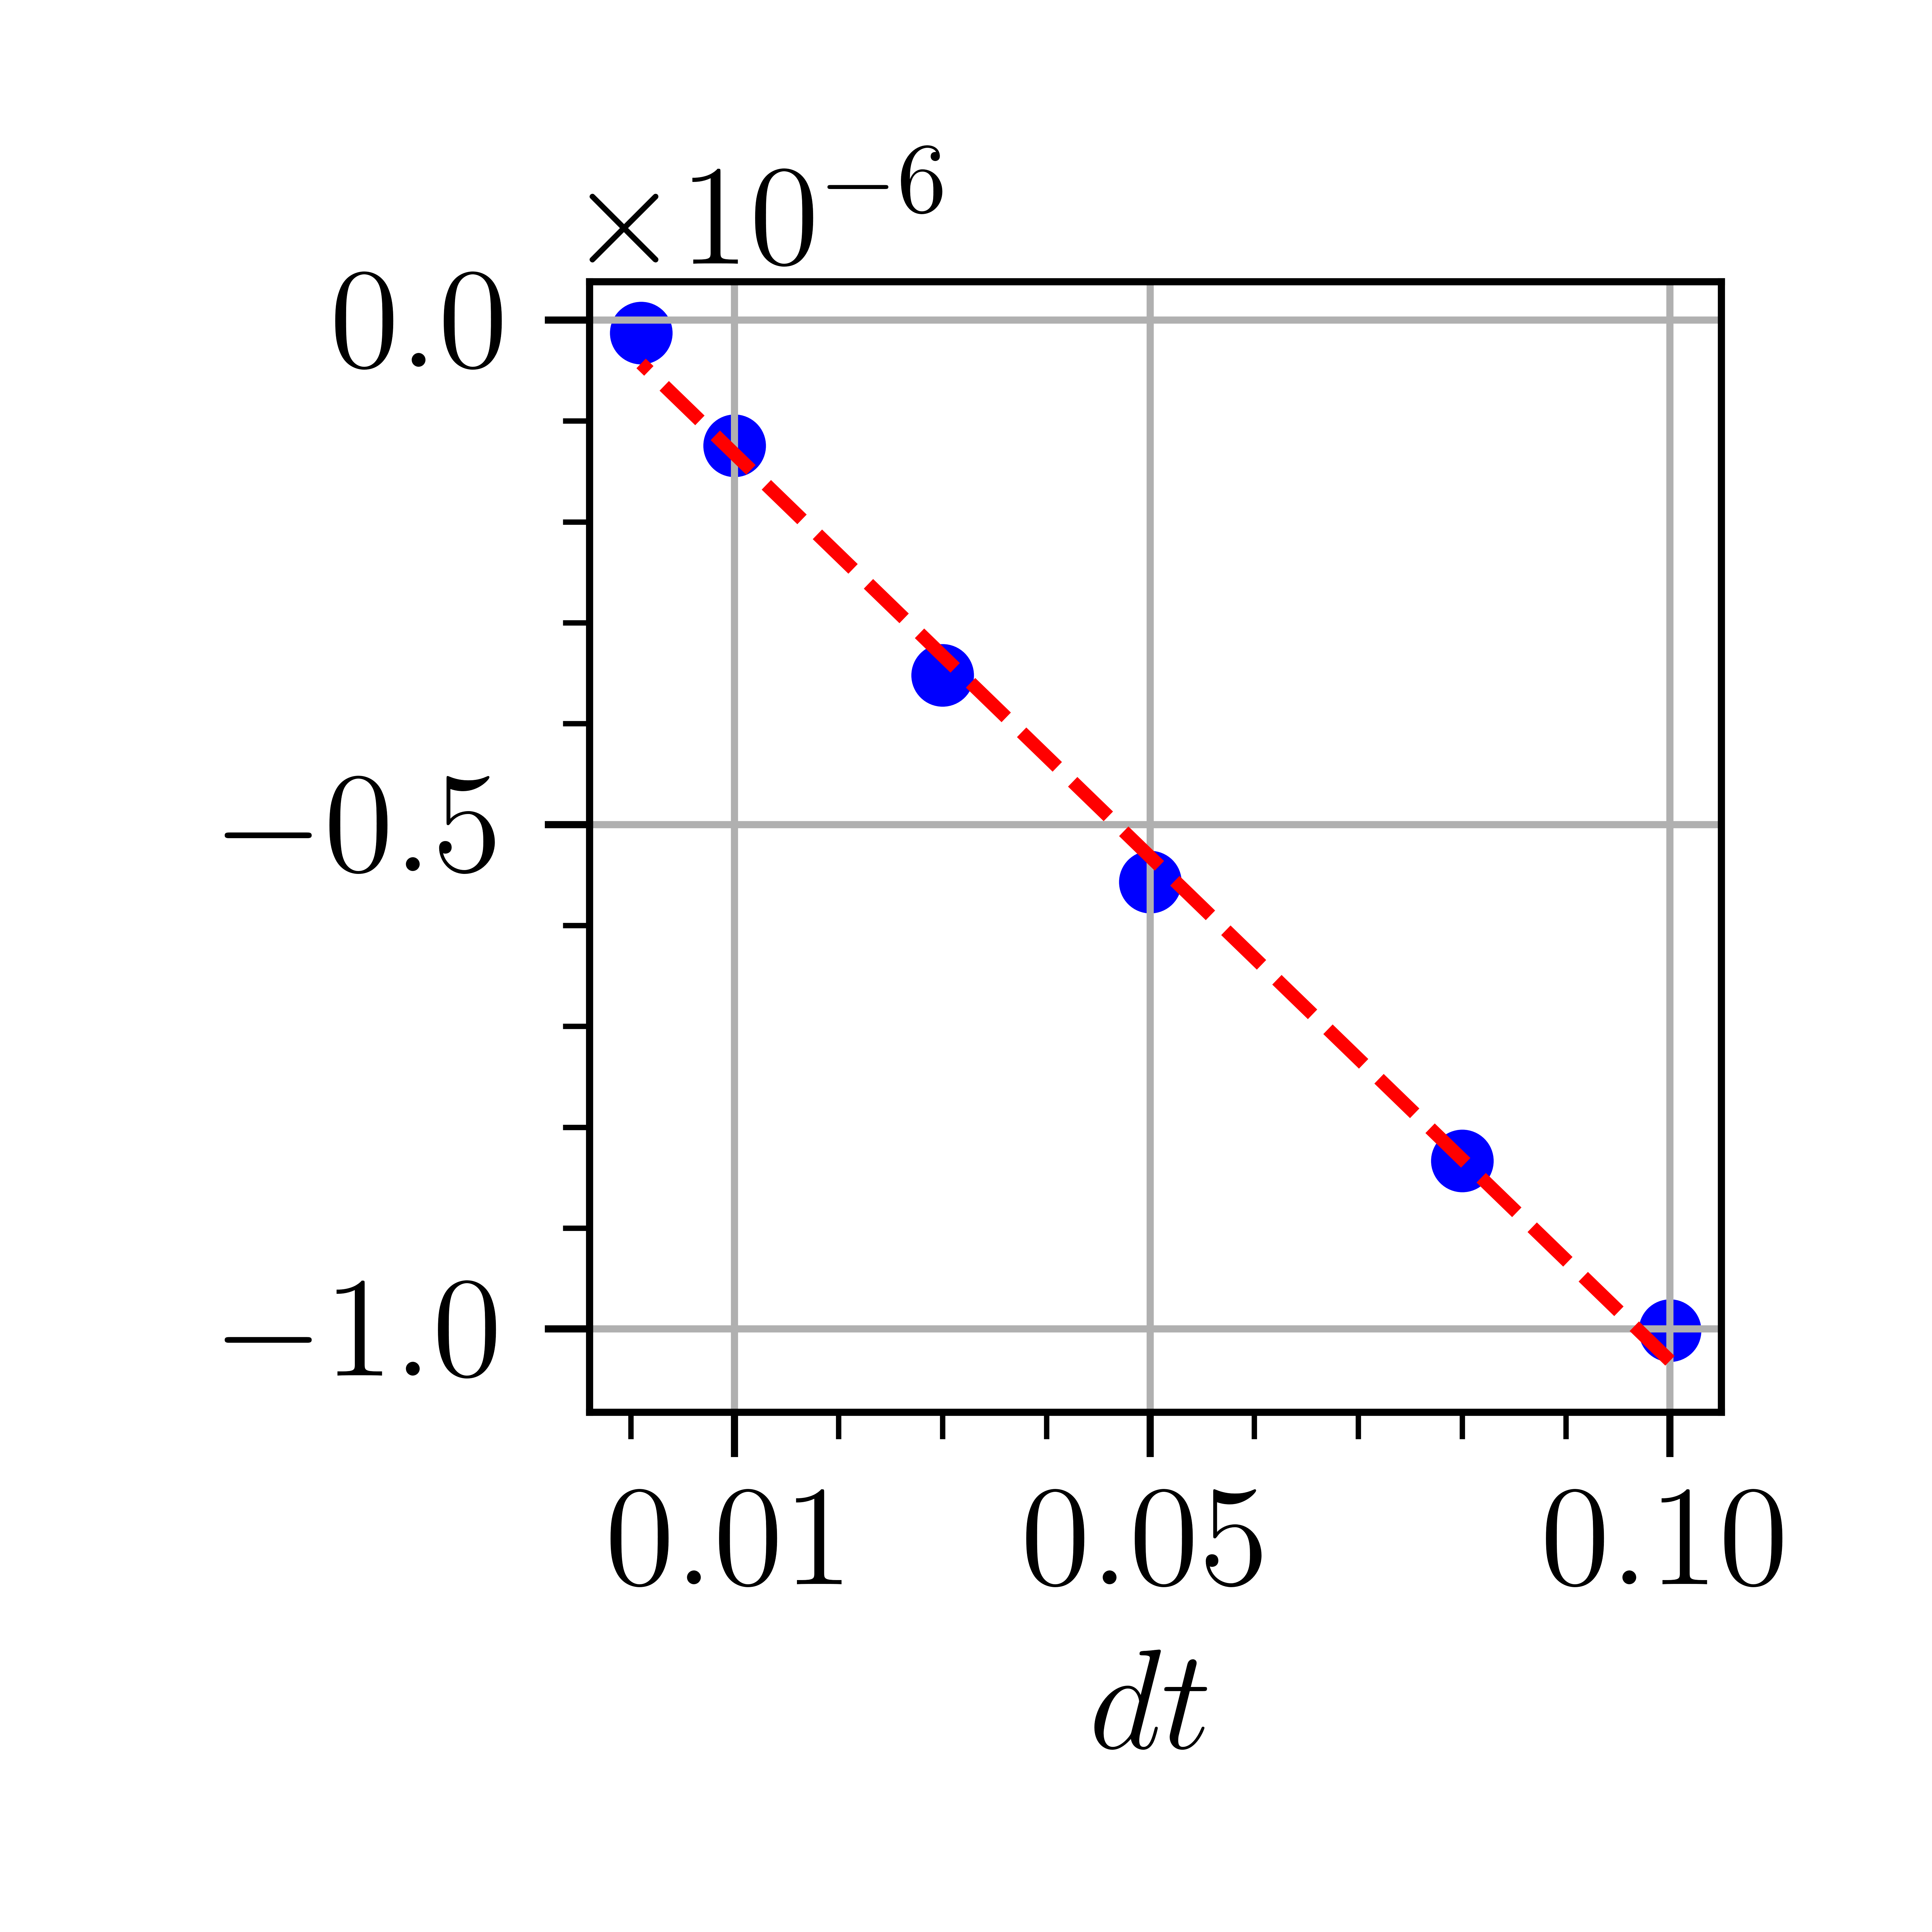
\includegraphics[width=1.0\textwidth]{figures/energy_conservation_euler_back}
	\caption{Euler Back method}
	\label{fig:energy_cons_euler_backward}
	\end{subfigure}
	\hfill
	\begin{subfigure}[b]{0.3\textwidth}
	\centering
	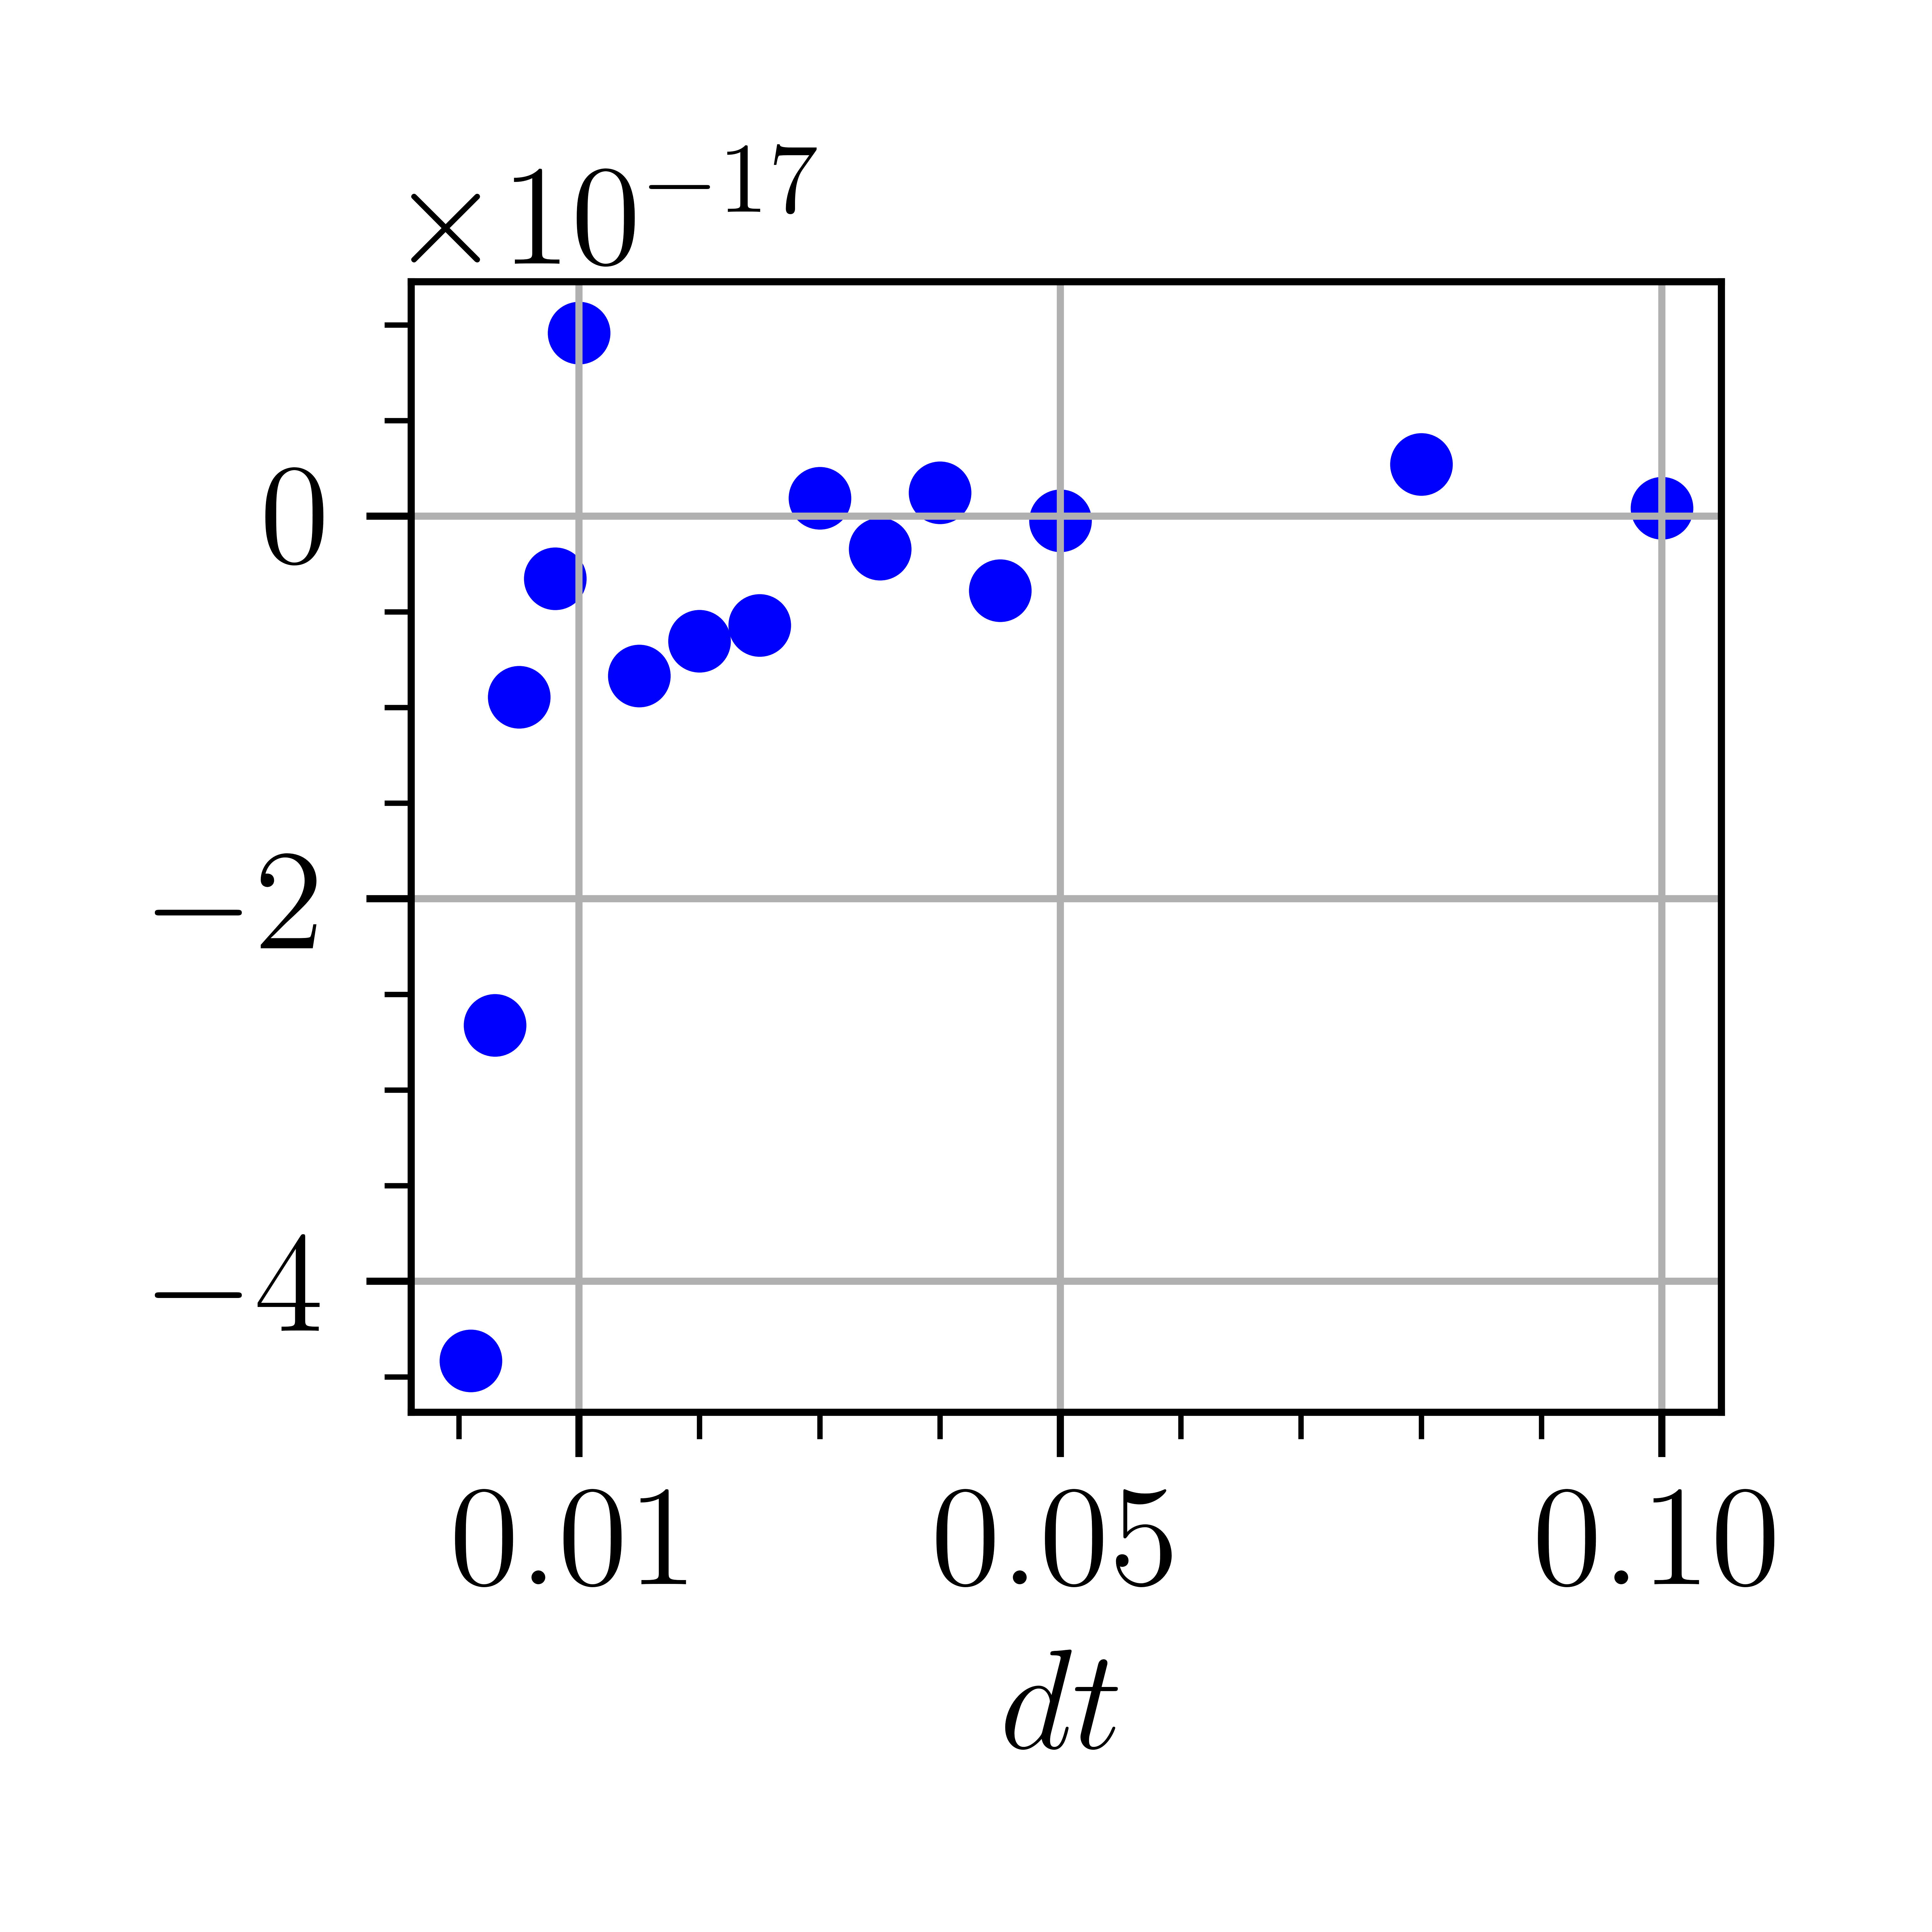
\includegraphics[width=1.0\textwidth]{figures/energy_conservation_rk4}
	\caption{RK4 method}
	\label{fig:energy_cons_rk4}
	\end{subfigure}	
	
	\caption{}Energy change slope compared against $dt$
	\label{fig:slopes-dt}
\end{figure}


The slopes in relation to the timestep $dt$ can be seen in fig. \ref{fig:slopes-dt}. For this given system, we find numerous notable finsings. Firstly, the Euler Back method is losing energy at a rate 2 magnitudes higher that that of the Euler method. This implies that the Euler method suits better in this particular system. 

Secondly does the RK4 integrator have a highly non-linear relationship \ref{fig:energy_cons_rk4} with some interesting features. In the range $0.03 \leq dt \leq 0.1$ is the relationship linear in nature, while letting the parameter become less than that it shows a spike, then going to the negative energy loss. Furthermore, a timestep of $0.1$ and $0.05$ is seemingly conserving the energy best by having the smallest change. One could argue here that the largest of the timesteps here is the most suitable.  

Lastly, it is important to note the difference in scales. Even though the first two methods show a linear relationship, RK4's energy change is in the magnitude of $10^{-17}$ compared to around $10^{-7}$ for the other two. 

(INSERT RELATIONSHIP)

Continuing, by taking a closer look at the energy with respect to time of the different models, some interesting behavior can be note. 

(INSERT ENERGY PLOTS FOR SHORT SYSTEM HERE)

Euler methdod and RK4 are both linear in nature, however, Euler Back is, in the time interval chosen here, oscillating. So taking a linear approximation of it may not be suitable. We now study a system where $T = 1000$. 

(INSERT ENERGY FOR LONG SYSTEM HERE)

We can see that the integrators are behaving similarily as before, only now there are some extra information that can be obtained from back euler. Studying the peaks and valleys, the amplitude is seemingly dissipating. Assuming that this dissipation is exponential, we can fit an exponential function to the peaks and valleys, and see what the energy converges to. (Note here that we could have ran the integration for long enough time, until the convergence is clear. However, setting $T=1000$ takes around 2 hrs. to complete, hence from time constraint, we will merely do analysis on the data available. 





